\documentclass[10pt,a4paper]{article}
\usepackage[utf8]{inputenc}
\usepackage[parfill]{parskip}
\usepackage[section]{placeins}
\usepackage{graphicx}
\usepackage{array}
\usepackage{tabularx}
\usepackage{apacite}
\usepackage{url}
\usepackage[left=3.00cm, right=3.00cm, top=3.00cm, bottom=3.00cm]{geometry}

\author{Christoph Emunds (i6146758)\\Richard Polzin (???)}
\title{Information Retrieval and Text Mining\\Emotion Mining and Topic Extraction on Lyrics}
\date{\today}

\begin{document}
	\maketitle
	
	\tableofcontents
	
	\section{Introduction}
	\label{sec:introduction}
	Measure the similarity of artists with respect to emotions and topics
	We give information about our dataset and how it was gathered
	Next, we describe the preprocessing that has been done on the data
	In the following two sections, we discuss the emotion mining and the topic extraction
	Afterwards, we show how the results have been visualized
	We explain the tools we used
	All of the processing is done in Python 3.6

	\section{Dataset}
	%100 top Billboard artists
	%20 metal bands from got-djent.com
	The \textit{pylyrics3} package is able to download the lyrics for all songs of a given artist if it exists on \textit{lyrics.wikia.com}. The lyrics are returned in a dictionary, where the keys are the song names and the values are the songs' lyrics. The usage of this package is straightforward and removes the necessity to deal with the raw HTML data. The retrieved songs are stored in JSON format, each song having a title, the artist's name and the actual lyrics.
	
	Some (how many?) of the top 100 Billboard artists could not be resolved when querying pylyrics3. This could be due to spelling variations. Moreover, we scraped the names of 30 metal bands from got-djent.com and requested their lyrics via pylyrics3. Some (how many?) of them could also not be resolved, either due to spelling variations or because they are not famous enough to have an entry in die LyricsWiki. Altogether, we ended up with 11.??? songs from 120 artists.

	In addition to the dataset we gathered ourselves we were given a database of more than 16.000 artists and 228.000 originally built by Sibirtsev and Schuster (???). In the remainder of this document, we call this dataset ???
	
	Some of the lyrics are not very clean. For example, they contain markers for the chorus and the verse part...

	\section{Preprocessing}	
	For tokenization and stemming, the \textit{nltk} Python package has been used. It provides easy to use function for splitting a document into sentences and splitting the sentences in words. Furthermore it implements several stemming algorithms. In our implementations, we use the Porter algorithm. We downloaded a list of stopwords that are more appropriate for lyrics. Moreover, in the process of topic extraction, we iteratively added words to this stopword list whenever we found...
	
	The tf-idf features are built with the help of the \textit{sklearn} package. It offers the \textit{TfIdfVectorizer} class, which...
	
	For the topic extraction, all songs should be in the same language, since otherwise the used algorithm will create an extra topic for every language.
	
	In our dataset, all songs, except for one, are in English. For the ??? dataset, we implemented a rudimentary language detection using the \textit{langdetect} Python package \cite{langdetect}. This package is a port of Google's language detection library.
	
	\section{Emotion Mining}
	NRC Emotion Lexicon (EmoLex)
	
		\subsection{Results}
		
		\begin{figure}[htb]
			\centering
			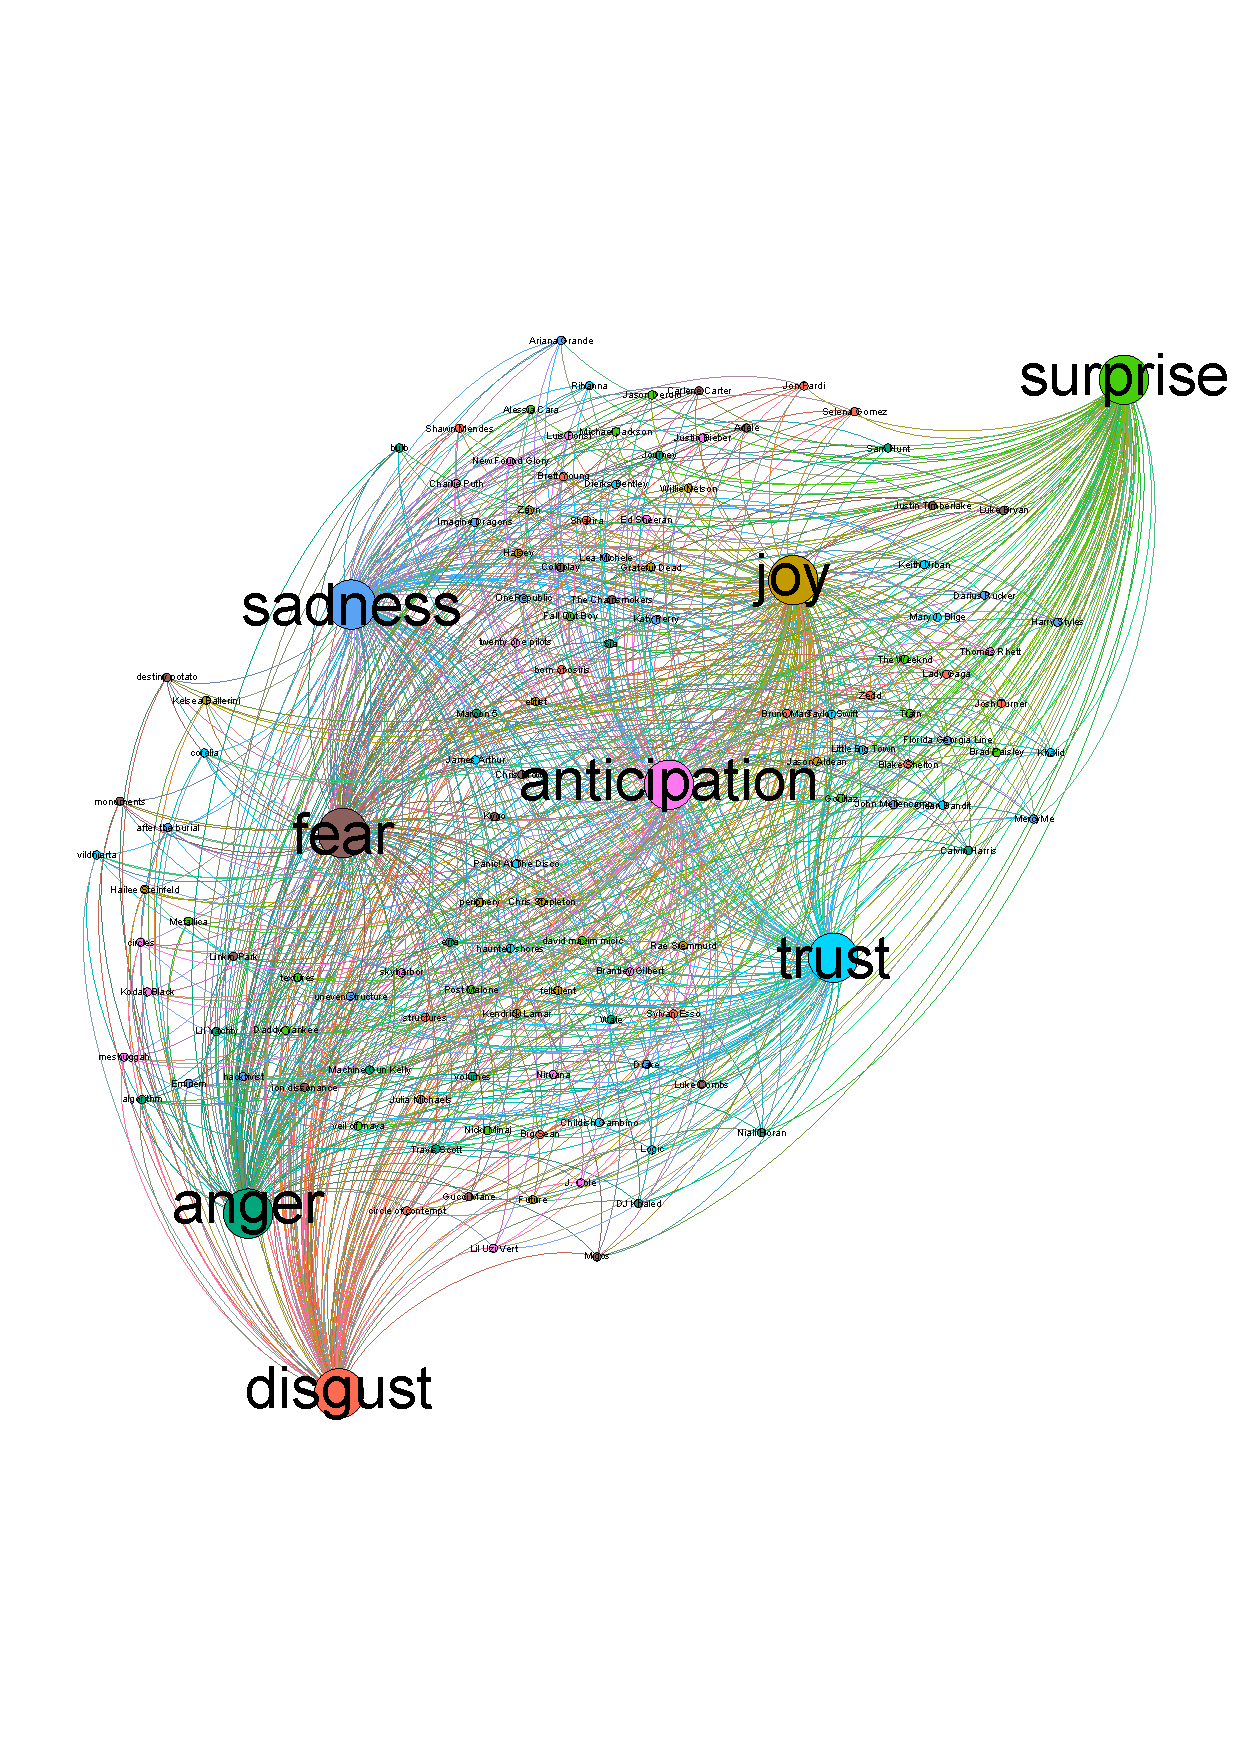
\includegraphics[trim=0mm 50mm 0mm 50mm, clip, width=0.7\linewidth]{data/emotion_clusters}
			\caption{Emotion clusters}
			\label{fig:emotionclusters}
		\end{figure}
	
	\section{Topic Extraction}
	Non-negative Matrix Factorization (NMF)
	Extracted 10 topics
	
		\subsection{Results}
	
	\section{Other techniques}
	RAKE
	Summarization
	Text statistics (Flesch Score, etc.)
	
	\section{Visualization}
	Used Gephi to visualize the results as a graph
	The \textit{pygraphml} package was used to dump the extracted information to a GraphML file, that can be imported by Gephi.
	Calculate modularity classes in Gephi

	\section{Conclusion}
	
	\newpage
	
	\bibliography{rp}
	\bibliographystyle{apacite}
	
\end{document}